\documentclass[11pt, oneside]{article}   	% use "amsart" instead of "article" for AMSLaTeX format
\usepackage{geometry}                		% See geometry.pdf to learn the layout options. There are lots.
\geometry{letterpaper}                   		% ... or a4paper or a5paper or ... 
%\geometry{landscape}                		% Activate for for rotated page geometry
%\usepackage[parfill]{parskip}    		% Activate to begin paragraphs with an empty line rather than an indent
\usepackage{graphicx}				% Use pdf, png, jpg, or eps� with pdflatex; use eps in DVI mode
								% TeX will automatically convert eps --> pdf in pdflatex		
\usepackage{amssymb}
\usepackage{amsmath}

\title{Linear Approximation}
%\author{The Author}
%\section{}
% \subsection*{R code}
\date{}							% Activate to display a given date or no date

\graphicspath{{/Users/telliott_admin/Dropbox/Tex/png/}}

\usepackage{listings,relsize} 
\lstloadlanguages{R} 
\lstset{language=R,basicstyle=\smaller[1],commentstyle=\rmfamily\smaller, 
  showstringspaces=false,% 
  xleftmargin=4ex,literate={<-}{{$\leftarrow$}}1 {~}{{$\sim$}}1} 
\lstset{escapeinside={(*}{*)}}   % for (*\ref{ }*) inside lstlistings (S code)

% \begin{lstlisting}  \end{lstlisting}
% \begin{center} 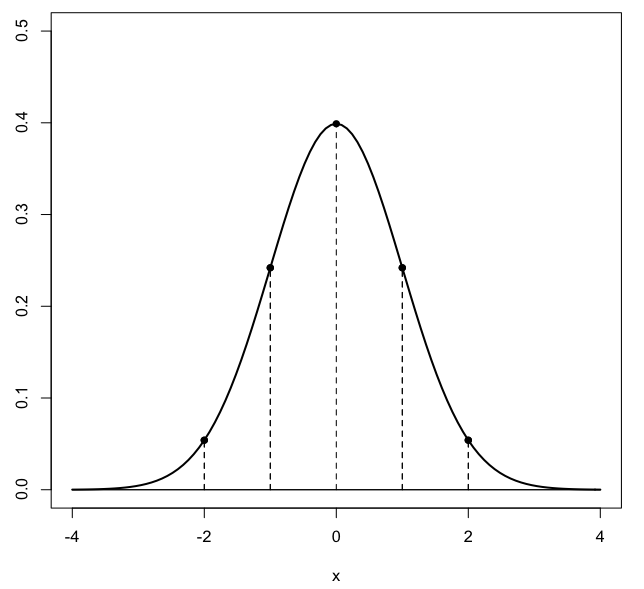
\includegraphics [scale=0.4] {gauss3.png} \end{center}
% \begin{bmatrix} a  &  b \\ c  &  d \end{bmatrix}
% \bigg |_

\begin{document}
\maketitle
\large
%\noindent
\begin{center} 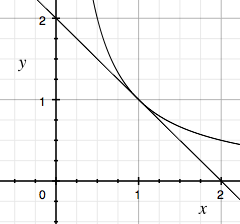
\includegraphics [scale=0.75] {linapprox1.png} \end{center}
Consider the branch of the hyperbola $xy=1$ for $x > 0$, in the first quadrant.  Pick a point $x_0,y_0$---in the figure it is at $P=(1,1)$ but it could be anywhere on the curve.  The linear approximation to the curve at $P$ is the line that goes through $P$ and which has the same slope as the curve does at $P$.
\[ f'(x) = \frac{d}{dx} \ \frac{1}{x} = -\frac{1}{x^2} = -\frac{1}{x_0^2} \ \ (\text{at} \ x_0) \]

\noindent
The equation of the line with this slope and going through $P$ is
\[ y - y_0 = -\frac{1}{x_0^2} (x - x_0) \]
Let's find the x-intercept ($y = 0$).
\[ - y_0 = -\frac{1}{x_0^2} (x - x_0) \]
But remember that $y_0 = 1/x_0$!
\[ -\frac{1}{x_0} = -\frac{1}{x_0^2} (x - x_0) \]
\[ 1 = \frac{1}{x_0} (x - x_0) \]
\[ x_0 = x - x_0 \]
\[ x = 2x_0 \]
We could do a similar calculation to find the y-intercept, but life is too short.  By symmetry, $x$ and $y$ can be interchanged, so
\[ y = 2y_0 \]
And now a neat result is that the area of the triangle determined by this line and the two axes is
\[ A = \frac{1}{2} \ 2x_0 \ 2y_0 =  2x_0 y_0 = 2 \]
The area is the same no matter which point $P$ we pick.  Maybe you could sketch a couple of these lines to check the result.


\end{document}  